\begin{center}
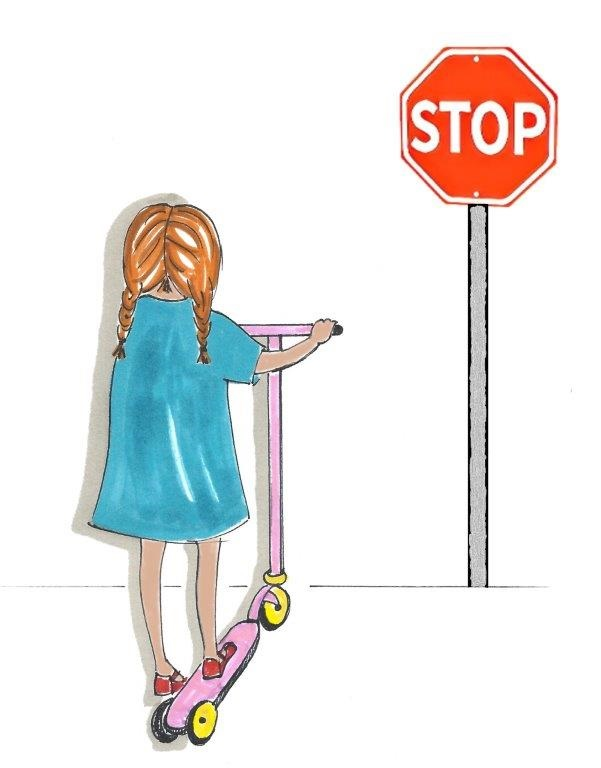
\includegraphics[width=0.4\textwidth]{content/3/chapter6/images/22.png}\\
Cippi在停车标志前停了下来
\end{center}

中断线程的功能是基于std::stop\_token、std::stop\_callback和std::stop\_source实现。

首先,杀死线程为什么不是一个好主意?

\begin{tcolorbox}[breakable,enhanced jigsaw,colback=red!5!white,colframe=red!75!black,title={杀死线程很危险}]
	
因为不知道线程当前的状态,可能会出现以下是两种的恶性结果。

\begin{itemize}
\item 
线程的工作只完成了一半。因为不知道它的作业的状态,所以也不知道程序的状态,从而以未定义的行为结束。

\item 
线程可能处于临界区,并且已经锁定了一个互斥锁。在线程锁定互斥锁时杀死线程,很可能导致死锁。
\end{itemize}
\end{tcolorbox}

\subsubsubsection{6.5.1\hspace{0.2cm} std::stop\_token, std::stop\_callback和std::stop\_source}

std::stop\_token、std::stop\_callback或std::stop\_source允许线程异步请求执行停止或查询一个执行是否得到了停止信号。std::stop\_token可以传递一个操作,然后用于主动轮询令牌,以获得停止请求或通过std::stop\_callback注册回调。停止请求由std::stop\_source发送,这个信号影响所有相关的std::stop\_token。std::stop\_source、std::stop\_token和std::stop\_callback三个类共享一个相关停止状态的所有权,request\_stop()、stop\_requested()和stop\_possible()是原子的。

可以用两种方法构造std::stop\_source:

\begin{lstlisting}[style=styleCXX]
stop_source();
explicit stop_source(std::nostopstate_t) noexcept;
\end{lstlisting}

默认构造函数(第1行)构造了一个std::stop\_source,其中包含一个新的停止状态。构造函数采用std::nostopstate\_t(第2行)构造一个空的std::stop\_source,没有相关的停止状态。

std::stop\_source src组件提供了以下成员函数来处理停止请求。

\begin{table}[H]
\centering
\begin{tabular}{ll}
\textbf{成员函数}       & \textbf{std::stop\_source src成员函数的描述}                                                                   \\ \hline
src.get\_token() &
\begin{tabular}[c]{@{}l@{}}若stop\_possible()为true,为相关的停止状态返回一个stop\_token。\\ 否则,返回一个默认构造的(空)stop\_token。\end{tabular} \\ \hline
src.stop\_possible()  & 若src可以请求停止,则为true。                                         \\ \hline
src.stop\_requested() & 若使用了stop\_possible()和request\_stop()中其中一个,则为true。 \\ \hline
src.request\_stop() &
\begin{tabular}[c]{@{}l@{}}若stop\_possible()和!stop\_requested(),则调用停止请求。\\否则,调用无效。\end{tabular} \\  \hline
\end{tabular}
\end{table}

src.stop\_possible()表示src有一个相关的停止状态。src.stop\_requested()在src有一个相关的停止状态并且之前没有要求停止时,返回true。使用src.request\_stop()是成功的,若src有一个相关的停止状态,并且之前没有请求停止,则返回true。

src.get\_token()返回停止令牌stoken。可以通过stoken检查停止请求是否已经发出,或可以为其相关的停止源src发出。停止标记stoken可以对停止源src进行观察。

\begin{table}[H]
\centering
\begin{tabular}{ll}
\textbf{成员函数} & \textbf{std::stop\_token stoken成员函数的描述}                                                                                                                   \\ \hline
stoken.stop\_possible()  & 若stoken有关联的停止状态,则返回true。                                                                                   \\ \hline
stoken.stop\_requested() & \begin{tabular}[c]{@{}l@{}}若在相关的std::stop\_source src上调用request\_stop(),则为true,\\ 否则为false。\end{tabular} \\  \hline
\end{tabular}
\end{table}

没有关联停止状态的默认构造令牌。若已经发出停止请求,stoken.stop\_possible也返回true。在停止令牌具有相关的停止状态,并且已经接收到停止请求时,stoken.stop\_requested()会返回true。

若std::stop\_token需要暂时禁用,可以用默认构造的令牌替换。默认构造的令牌没有关联的停止状态。下面的代码片段展示了如何禁用和启用线程接受停止请求的能力。

\hspace*{\fill} \\ %插入空行
\noindent
\textbf{暂时禁用停止令牌}
\begin{lstlisting}[style=styleCXX]
std::jthread jthr([](std::stop_token stoken) {
	...
	std::stop_token interruptDisabled;
	std::swap(stoken, interruptDisabled);
	...
	std::swap(stoken, interruptDisabled);
	...
}
\end{lstlisting}

std::stop\_token interruptDisabled没有关联的停止状态,所以线程jthr可以接受除第4和第5行以外的所有行中的停止请求。

下一个例子展示了如何使用回调。

\begin{lstlisting}[style=styleCXX]
// invokeCallback.cpp

#include <atomic>
#include <chrono>
#include <iostream>
#include <thread>
#include <vector>

using namespace std::literals;

auto func = [](std::stop_token stoken) {
		std::atomic<int> counter{0};
		auto thread_id = std::this_thread::get_id();
		std::stop_callback callBack(stoken, [&counter, thread_id] {
			std::cout << "Thread id: " << thread_id
					  << "; counter: " << counter << '\n';
		});
		while (counter < 10) {
			std::this_thread::sleep_for(0.2s);
			++counter;
		}
	};

int main() {

	std::cout << '\n';
	
	std::vector<std::jthread> vecThreads(10);
	for(auto& thr: vecThreads) thr = std::jthread(func);
	
	std::this_thread::sleep_for(1s);
	
	for(auto& thr: vecThreads) thr.request_stop();
	
	std::cout << '\n';

}
\end{lstlisting}

这十个线程中的每一个都调用Lambda函数func(第11-22行),第14-17行中的回调显示线程id和计数器。由于主线程的休眠时间为1秒,子线程的休眠时间为1秒,因此调用回调时计数器为4。thr.request\_stop()在每个线程上都会触发回调。

\begin{center}
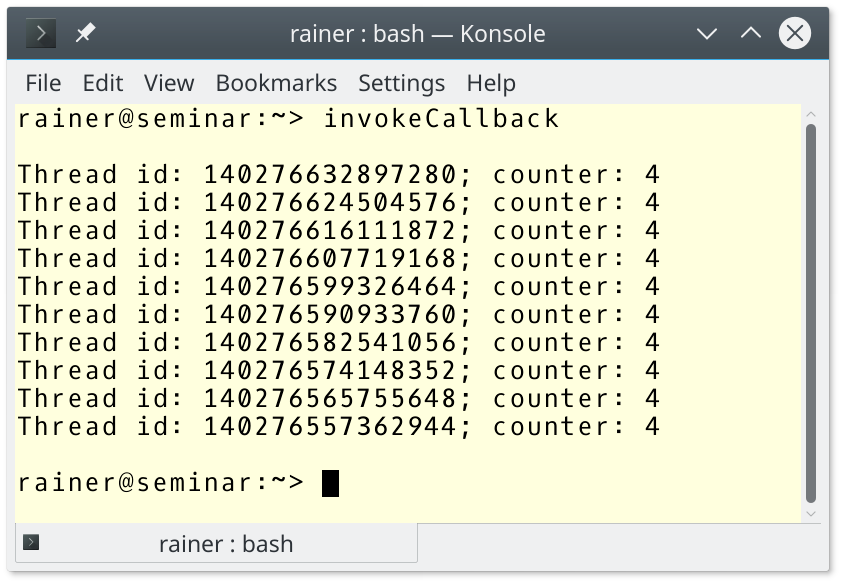
\includegraphics[width=0.6\textwidth]{content/3/chapter6/images/23.png}\\
\end{center}

\hspace*{\fill} \\ %插入空行
\noindent
\textbf{6.5.1.1\hspace{0.2cm}汇入线程}

std::jthread是一个std::thread,其功能就是可以发出中断信号和自动join()。为了支持这个功能,其具有一个std::stop\_token。

\begin{table}[H]
\centering
\begin{tabular}{ll}
\textbf{成员函数}   & \textbf{std::jthread jthr用于停止令牌处理成员函数的描述}                                        \\ \hline
t.get\_stop\_source() & 返回与共享停止状态关联的std::stop\_source对象。 \\
t.get\_stop\_token()  & 返回与共享停止状态关联的std::stop\_token对象。  \\
t.request\_stop() & 通过共享停止状态停止执行请求。
\end{tabular}
\end{table}

\hspace*{\fill} \\ %插入空行
\noindent
\textbf{6.5.1.2\hspace{0.2cm}condition\_variable\_any的新重载}

std::condition\_variable\_any的三个wait变量的wait、wait\_for和wait\_until得到新的重载,都有一个std::stop\_token。

\begin{lstlisting}[style=styleCXX]
template <class Predicate>
bool wait(Lock& lock,
		stop_token stoken,
		Predicate pred);

template <class Rep, class Period, class Predicate>
bool wait_for(Lock& lock,
			stop_token stoken,
			const chrono::duration<Rep, Period>& rel_time,
			Predicate pred);

template <class Clock, class Duration, class Predicate>
bool wait_until(Lock& lock,
			stop_token stoken,
			const chrono::time_point<Clock, Duration>& abs_time,
			Predicate pred);
\end{lstlisting}

这些新的重载需要一个谓词,所提供的版本需要确保线程在对传递的std::stop\_token stoken的停止请求发出信号时得到通知。其会返回一个布尔值,指示谓词的结果是否为true。返回的布尔值与是否请求停止或是否触发超时无关。这三个重载等价于以下表达式:

\begin{lstlisting}[style=styleCXX]
// wait in lines 1 - 4
while (!stoken.stop_requested()) {
	if (pred()) return true;
	wait(lock);
}
return pred();

// wait_for in lines 6 - 10
return wait_until(lock,
					std::move(stoken),
					chrono::steady_clock::now() + rel_time,
					std::move(pred)
					);

// wait_until in lines 12 - 16
while (!stoken.stop_requested()) {
	if (pred()) return true;
	if (wait_until(lock, timeout_time) == std::cv_status::timeout) return pred();
}
return pred();
\end{lstlisting}

等待调用之后,可以检查是否有停止请求。

\begin{lstlisting}[style=styleCXX]
cv.wait(lock, stoken, predicate);
if (stoken.stop_requested()){
	// interrupt occurred
}
\end{lstlisting}

下面的示例展示了条件变量与停止请求的使用方式。

\begin{lstlisting}[style=styleCXX]
// conditionVariableAny.cpp

#include <condition_variable>
#include <thread>
#include <iostream>
#include <chrono>
#include <mutex>
#include <thread>

using namespace std::literals;

std::mutex mut;
std::condition_variable_any condVar;

bool dataReady;

void receiver(std::stop_token stopToken) {

	std::cout << "Waiting" << '\n';
	
	std::unique_lock<std::mutex> lck(mut);
	bool ret = condVar.wait(lck, stopToken, []{return dataReady;});
	if (ret){
		std::cout << "Notification received: " << '\n';
	}
	else{
		std::cout << "Stop request received" << '\n';
	}
}

void sender() {

	std::this_thread::sleep_for(5ms);
	{
		std::lock_guard<std::mutex> lck(mut);
		dataReady = true;
		std::cout << "Send notification" << '\n';
	}
	condVar.notify_one();

}

int main(){

	std::cout << '\n';
	
	std::jthread t1(receiver);
	std::jthread t2(sender);
	
	t1.request_stop();
	
	t1.join();
	t2.join();
	
	std::cout << '\n';

}
\end{lstlisting}

接收线程(第17-29行)正在等待发送线程(第31-41行)的通知。发送方线程在第39行发送通知之前,主线程在第50行触发了一个停止请求。程序的输出显示,停止请求发生在通知之前。

\begin{tcblisting}{commandshell={}}
Waiting
Stop request received
Send notification
\end{tcblisting}

\begin{tcolorbox}[breakable,enhanced jigsaw,colback=mygreen!5!white,colframe=mygreen!75!black,title={总结}]
	
\begin{itemize}
\item 
可以使用std::stop\_token、std::stop\_source和std::stop\_callback,对线程和条件变量进行协作中断。协作中断意味着线程获得一个可以接受或忽略的停止请求。

\item 
std::stop\_token可以传递给一个操作,用来主动轮询令牌以获得停止请求,或者使用std::stop\_callback注册一个回调。

\item 
除了std::jthread之外,std::condition\_variable\_any也可以接受停止请求。
\end{itemize}
	
\end{tcolorbox}



\newpage















